\documentclass[aspectratio=169,11pt]{beamer}

% ---- Theme & colors ----
\usetheme{default}
\usecolortheme{default}
\useinnertheme{circles}
\setbeamertemplate{navigation symbols}{}
\setbeamertemplate{itemize items}[circle]

\definecolor{UPAblue}{HTML}{1F77B4}
\definecolor{BPAorange}{HTML}{E8823A}
\definecolor{darkink}{HTML}{1A2B3C}
\definecolor{softgray}{HTML}{6B7280}

\setbeamercolor{frametitle}{fg=white,bg=UPAblue}
\setbeamercolor{title}{fg=UPAblue}
\setbeamercolor{structure}{fg=UPAblue}
\setbeamercolor{alerted text}{fg=BPAorange}
\setbeamerfont{frametitle}{series=\bfseries}
\setbeamerfont{title}{series=\bfseries}

\usepackage{amsmath,amssymb}
\usepackage{booktabs}
\usepackage{graphicx}
\usepackage{tikz}

% frame-title bar spacing
\setbeamertemplate{frametitle}{%
  \nointerlineskip
  \begin{beamercolorbox}[wd=\paperwidth,ht=2.6ex,dp=1.2ex,leftskip=0.3cm,rightskip=0.3cm]{frametitle}%
    \usebeamerfont{frametitle}\insertframetitle%
  \end{beamercolorbox}%
}

\newcommand{\take}[1]{\vspace{0.3em}\begin{beamercolorbox}[wd=\textwidth,sep=6pt,rounded=true]{block body}\color{darkink}\small\textbf{Takeaway:} #1\end{beamercolorbox}}

% ---- Title metadata ----
\title{Optimization-Based Clinical Decision Support for Curable Hypertension}
\subtitle{SVMs: Hard-Margin Feasibility, Soft Margins, and Kernel Validation}
\author{Nguyen Thanh Tung \and Duong Van Khoa}
\institute{Optimization for Data Science Project \\ Singapore University of Technology and Design}
\date{\today}

\begin{document}

% ---------- Title ----------
\begin{frame}[plain]
  \titlepage
\end{frame}

% ---------- Roadmap ----------
\begin{frame}{The story in one line}
  \vspace{0.5em}
  \begin{center}
    \large
    \textcolor{UPAblue}{\textbf{strict}}
    $\,\rightarrow\,$
    \textcolor{BPAorange}{\textbf{prove impossible}}
    $\,\rightarrow\,$
    \textcolor{UPAblue}{\textbf{relax}}
    $\,\rightarrow\,$
    \textcolor{BPAorange}{\textbf{compare}}
    $\,\rightarrow\,$
    \textcolor{UPAblue}{\textbf{conclude}}
  \end{center}
  \vspace{1em}
  \begin{itemize}
    \item Try the \textbf{hard-margin} SVM: a straight line with zero mistakes.
    \item \textbf{Prove} no such line exists --- three independent ways.
    \item \textbf{Relax} to a soft margin that charges for mistakes.
    \item \textbf{Compare} against a curved (RBF kernel) boundary.
    \item \textbf{Conclude}: the simple linear model is the right choice.
  \end{itemize}
\end{frame}

% ---------- Problem ----------
\begin{frame}{The clinical problem}
  \begin{columns}[T]
    \begin{column}{0.58\textwidth}
      \textbf{Primary aldosteronism (PA)} is a common, \emph{curable} cause of high blood pressure.
      \vspace{0.6em}
      \begin{itemize}
        \item \textcolor{UPAblue}{\textbf{Unilateral (UPA)}}: one gland --- often \emph{cured by surgery}.
        \item \textcolor{BPAorange}{\textbf{Bilateral (BPA)}}: both glands --- managed with \emph{medication}.
      \end{itemize}
      \vspace{0.6em}
      Getting the subtype right changes the treatment. Can an optimization model separate the two from routine measurements?
    \end{column}
    \begin{column}{0.40\textwidth}
      \begin{block}{The dataset}
        \small
        \begin{itemize}
          \item 114 synthetic patients
          \item 56 UPA \; / \; 58 BPA
          \item 10 continuous predictors\\{\footnotesize (PAC, PRA, potassium, tumor size, steroids, BP, \ldots)}
        \end{itemize}
      \end{block}
    \end{column}
  \end{columns}
  \take{Frame subtype classification as a maximum-margin optimization problem.}
\end{frame}

% ---------- Descriptive statistics ----------
\begin{frame}{What the data look like before any model}
  \centering
  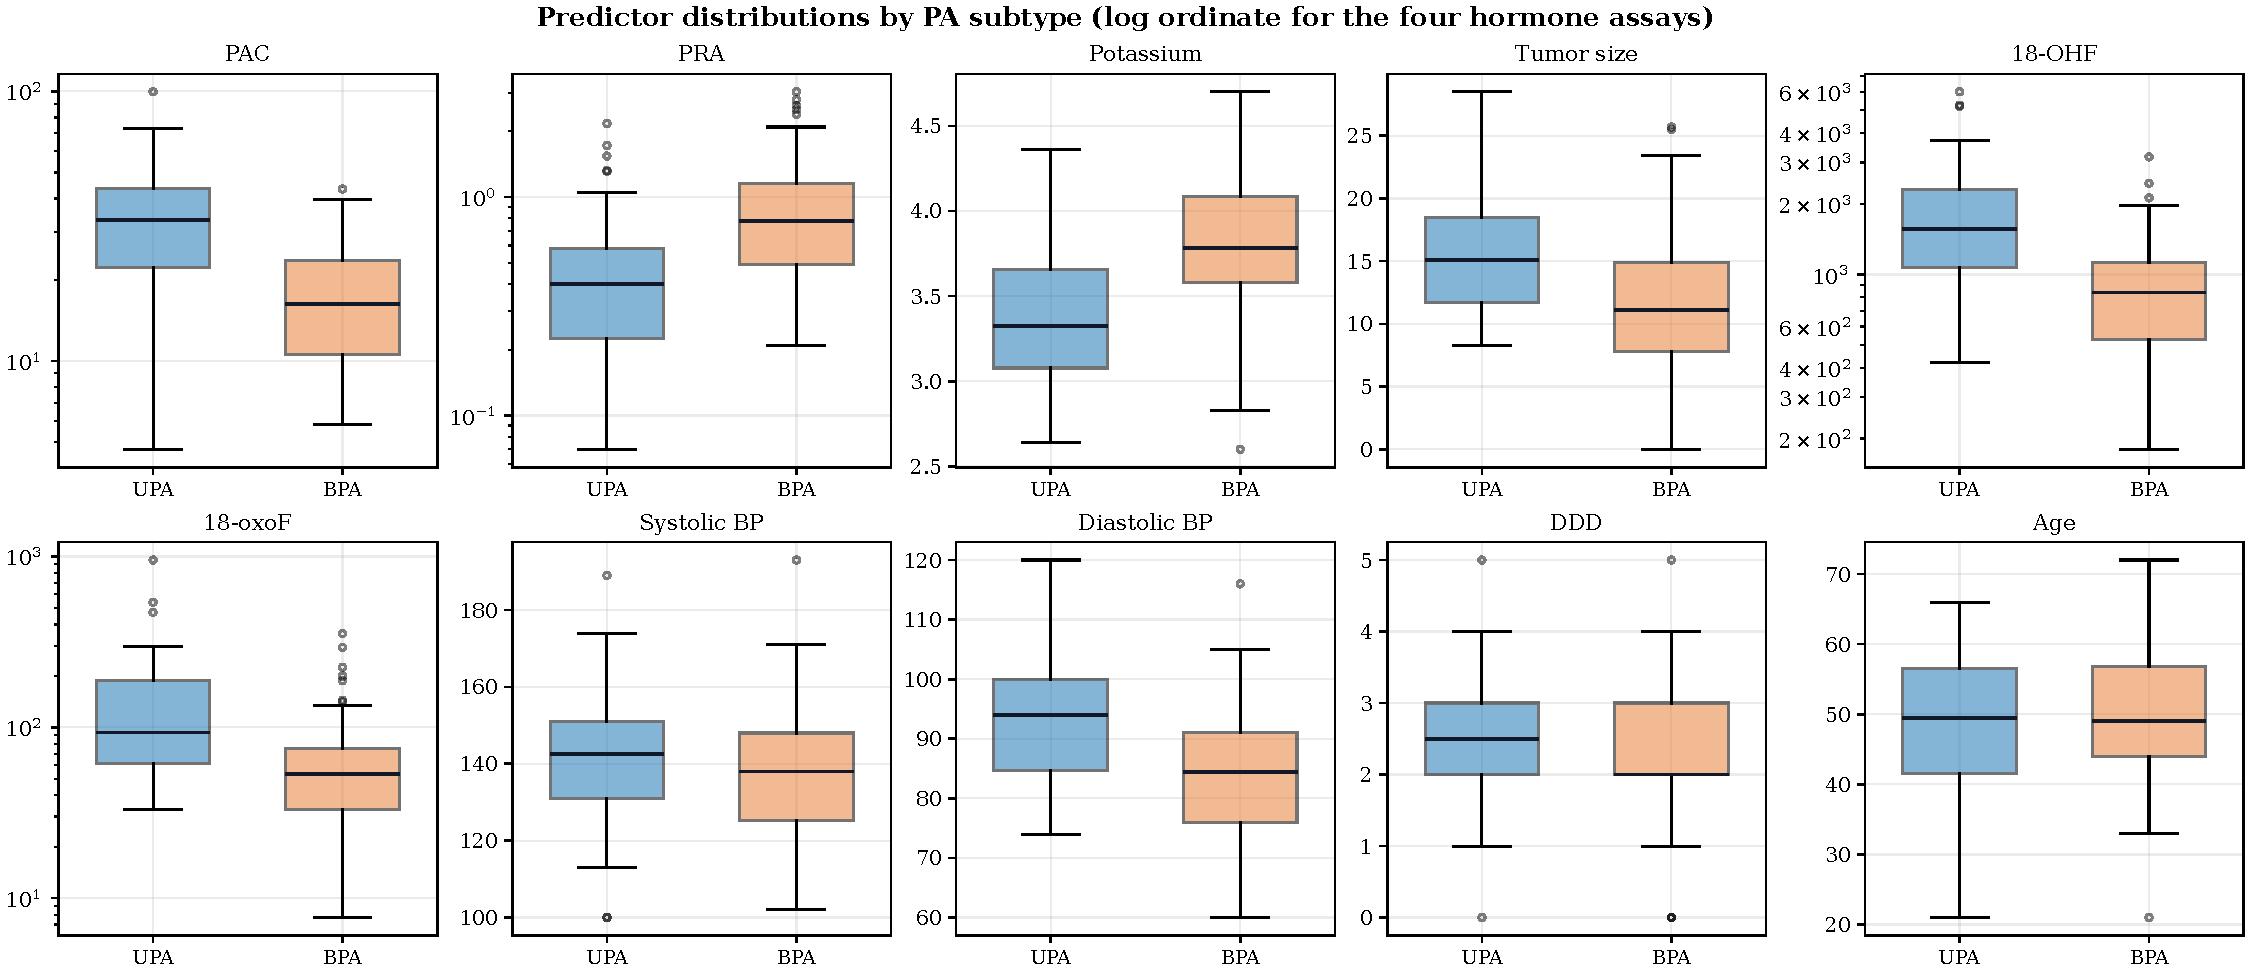
\includegraphics[width=0.80\textwidth]{output/figures/feature_distributions.pdf}
  \\[0.15em]
  {\footnotesize 114 patients, no missing values.
  \textcolor{UPAblue}{\textbf{UPA}} versus \textcolor{BPAorange}{\textbf{BPA}};
  hormone assays on a log ordinate.}
  \take{Every panel overlaps --- no single measurement splits the two subtypes.}
\end{frame}

\begin{frame}{Descriptive statistics --- the subtype contrast}
  \begin{columns}[T]
    \begin{column}{0.58\textwidth}
      \scriptsize
      \setlength{\tabcolsep}{3.5pt}
      \begin{tabular}{lccrr}
        \toprule
        Feature & UPA & BPA & Cohen's $d$ & Welch $t$ \\
        \midrule
        PAC (ng/dL)      & 34.9  & 18.4  & \textbf{1.17} & \textbf{6.20} \\
        18-OHF (ng/dL)   & 1883  & 942   & \textbf{0.99} & \textbf{5.25} \\
        Potassium (mmol/L) & 3.38 & 3.79 & \textbf{-0.95} & \textbf{-5.09} \\
        PRA (ng/mL/h)    & 0.51  & 0.96  & \textbf{-0.80} & \textbf{-4.32} \\
        Diastolic BP (mmHg) & 92.3 & 84.1 & \textbf{0.75} & \textbf{4.03} \\
        Tumor size (mm)  & 15.4  & 11.4  & \textbf{0.74} & \textbf{3.98} \\
        18-oxoF (ng/dL)  & 148.1 & 71.8  & \textbf{0.66} & \textbf{3.46} \\
        \midrule
        DDD (drugs)      & 2.48  & 2.14  & 0.36 & 1.94 \\
        Systolic BP (mmHg) & 141.4 & 137.5 & 0.23 & 1.22 \\
        Age (years)      & 48.6  & 50.1  & -0.15 & -0.80 \\
        \bottomrule
      \end{tabular}
      \\[0.4em]
      {\tiny Bold: $|t|>2$, i.e.\ separates the subtypes (7 of 10).
      Sign: $+$ means higher in UPA.}
    \end{column}
    \begin{column}{0.40\textwidth}
      \begin{block}{Cohen's $d$ --- how big}
        \small
        Gap between \emph{class means}, in pooled SDs:
        $0.2$ small, $0.5$ medium, $0.8+$ large.
      \end{block}
      \begin{block}{Welch $t$ --- how certain}
        \small
        Same gap $\div$ standard error; grows with $\sqrt{n}$.
        Evidence, not size.
      \end{block}
    \end{column}
  \end{columns}
  \take{Strong univariate signal, but overlapping distributions --- a perfect separator is in doubt.}
\end{frame}

% ---------- Hard margin geometry ----------
\begin{frame}{Step 1 --- the strictest model: hard-margin SVM}
  \begin{columns}[T]
    \begin{column}{0.48\textwidth}
      Find the \textbf{widest empty corridor} between the two classes:
      \[
        \min_{w,b}\ \tfrac12\lVert w\rVert^2
        \quad\text{s.t.}\quad t_i(w^\top x_i+b)\ge 1.
      \]
      \begin{itemize}
        \item Score $s=w^\top x+b$; sign is the prediction.
        \item Margin width $=2/\lVert w\rVert$.
        \item \textbf{Zero mistakes allowed.}
      \end{itemize}
      A convex quadratic program --- \emph{if} a feasible line exists.
    \end{column}
    \begin{column}{0.52\textwidth}
      \centering
      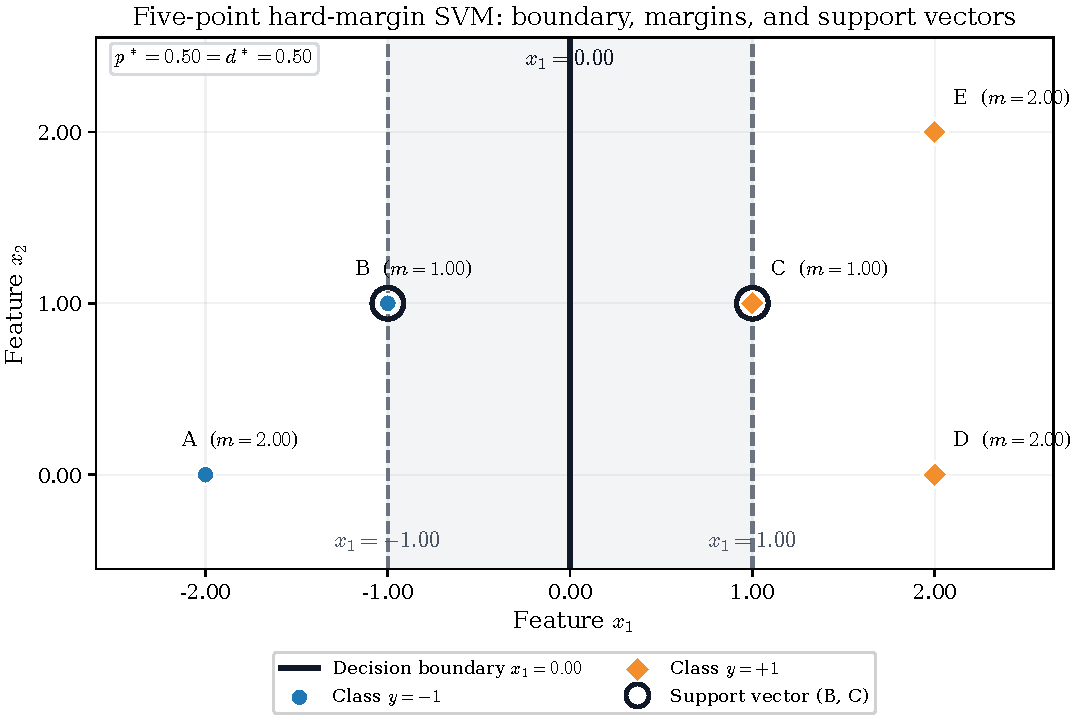
\includegraphics[width=\textwidth]{output/figures/svm_primal_dual_toy_example.pdf}\\
      {\footnotesize Five-point teaching example: boundary, margins, support vectors.}
    \end{column}
  \end{columns}
\end{frame}

% ---------- Infeasibility ----------
\begin{frame}{Step 2 --- prove no such line exists}
  \vspace{0.4em}
  We attack the question \alert{three independent ways}. If any one succeeds, the hard-margin model is impossible --- and all three agree.
  \vspace{0.8em}
  \begin{columns}[T]
    \begin{column}{0.33\textwidth}
      \begin{block}{2a. Ask the solver}
        \small Run the feasibility LP on all data and every fold.
      \end{block}
    \end{column}
    \begin{column}{0.33\textwidth}
      \begin{block}{2b. Farkas certificate}
        \small Get a signed receipt --- 12 patients that \emph{prove} $0\ge1$.
      \end{block}
    \end{column}
    \begin{column}{0.33\textwidth}
      \begin{block}{2c. Convex hulls}
        \small Show the two classes literally share a point.
      \end{block}
    \end{column}
  \end{columns}
  \vspace{0.9em}
  \begin{center}
    \small Each is stronger than the last: a solver \emph{says} no; Farkas \emph{proves} no; the hulls \emph{show} why.
  \end{center}
\end{frame}

% ---------- 2a solver ----------
\begin{frame}{Step 2a --- ask the solver}
  \begin{columns}[T]
    \begin{column}{0.52\textwidth}
      Feasibility of the hard-margin constraints is itself a \textbf{linear program}: does any $(w,b)$ satisfy
      \[
        t_i(w^\top x_i + b)\ge 1 \quad\text{for all } i?
      \]
      \begin{itemize}
        \item HiGHS returns \alert{\textbf{status: infeasible}} on the full 114-patient dataset.
        \item Repeated inside every one of the 5 cross-validation folds --- \textbf{all infeasible}.
        \item So the result is not an artifact of one particular split.
      \end{itemize}
    \end{column}
    \begin{column}{0.48\textwidth}
      \centering
      \begin{block}{Solver verdict}
        \footnotesize
        \begin{tabular}{ll}
          \toprule
          Subset & Feasible? \\
          \midrule
          Full data (114) & \textcolor{BPAorange}{\textbf{No}} \\
          Fold 1 & \textcolor{BPAorange}{\textbf{No}} \\
          Fold 2 & \textcolor{BPAorange}{\textbf{No}} \\
          Fold 3 & \textcolor{BPAorange}{\textbf{No}} \\
          Fold 4 & \textcolor{BPAorange}{\textbf{No}} \\
          Fold 5 & \textcolor{BPAorange}{\textbf{No}} \\
          \bottomrule
        \end{tabular}
      \end{block}
    \end{column}
  \end{columns}
  \take{A ``no'' from the solver is a starting point --- but why should we trust it? Steps 2b--2c give proof.}
\end{frame}

% ---------- 2b Farkas ----------
\begin{frame}{Step 2b --- the Farkas certificate}
  \begin{columns}[T]
    \begin{column}{0.42\textwidth}
      \textbf{Farkas' lemma}: exactly \emph{one} of two systems can hold ---
      either a separating $w$ exists, \textbf{or} a set of nonnegative weights $\lambda$ gives a contradiction.
      \vspace{0.5em}
      \begin{itemize}
        \item The solver hands back \textbf{12 patients} with weights $\lambda_i\ge0$.
        \item They combine to prove $0\ge 1$ --- impossible.
        \item This is a \emph{checkable receipt}: no need to trust the solver's search.
      \end{itemize}
    \end{column}
    \begin{column}{0.58\textwidth}
      \centering
      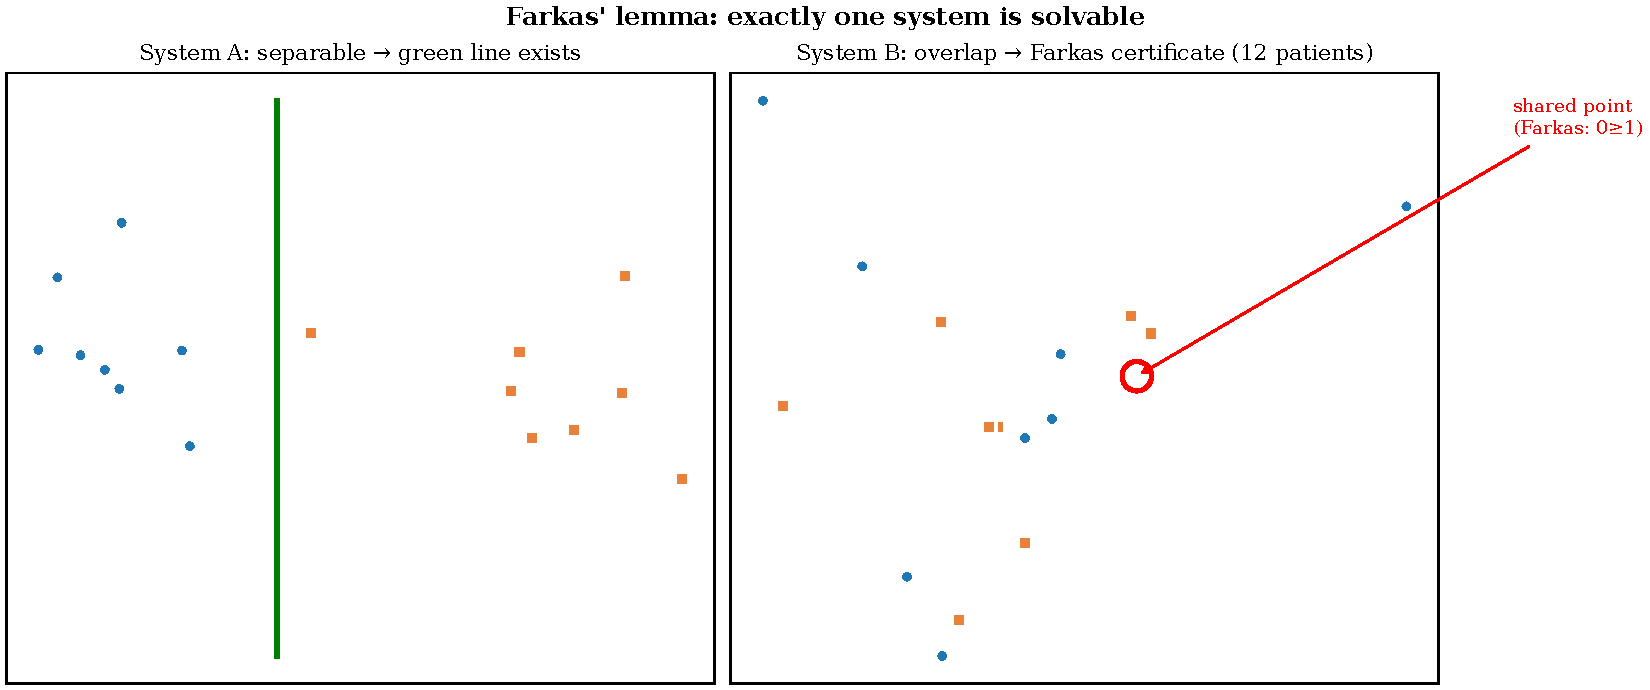
\includegraphics[width=\textwidth]{output/figures/farkas_lemma_schematic.pdf}\\
      {\footnotesize Only one column can be true. On this data it is the right one.}
    \end{column}
  \end{columns}
  \take{The certificate turns ``the solver said no'' into a proof anyone can verify by hand.}
\end{frame}

% ---------- 2c convex hull ----------
\begin{frame}{Step 2c --- what the certificate means: overlapping hulls}
  \begin{columns}[T]
    \begin{column}{0.42\textwidth}
      \small
      The same $\lambda$ weights have a picture. Rescaled, they build \textbf{one point inside both classes' convex hulls}:
      \[
        \textstyle\sum_i \beta_i^{+} x_i = \sum_i \beta_i^{-} x_i,
      \]
      matching to $6.66\times10^{-16}$ (machine zero).
      \begin{itemize}
        \item A shared point $\Rightarrow$ no hyperplane separates the classes.
        \item Geometry, solver, and algebra tell one story.
      \end{itemize}
    \end{column}
    \begin{column}{0.58\textwidth}
      \centering
      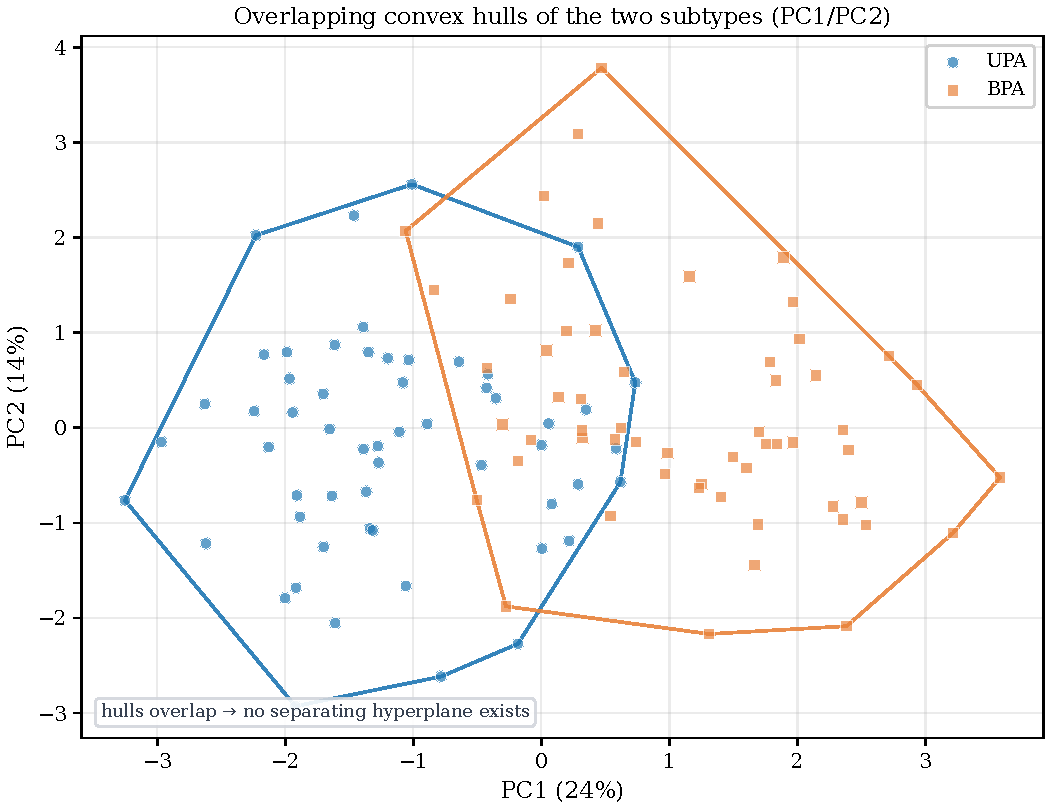
\includegraphics[width=\textwidth]{output/figures/convex_hull_overlap_2d.pdf}\\
      {\footnotesize The real cohort in a 2-D projection: the hulls clearly overlap. The full-dimensional proof is exact.}
    \end{column}
  \end{columns}
  \take{The hard-margin model is not a failed solve --- it is provably impossible on this data.}
\end{frame}

% ---------- Soft margin ----------
\begin{frame}{Step 3 --- relax: the soft-margin SVM}
  \begin{columns}[T]
    \begin{column}{0.46\textwidth}
      Allow mistakes, but \textbf{charge} for them with slack $\xi_i$:
      \[
        \min_{w,b,\xi}\ \tfrac12\lVert w\rVert^2 + C\!\sum_i \xi_i
      \]
      \[
        \text{s.t.}\ \ t_i(w^\top x_i+b)\ge 1-\xi_i,\ \ \xi_i\ge0.
      \]
      \begin{itemize}
        \item $C$ = strictness knob (chosen by nested CV).
        \item Selected \textbf{$C=0.01$} (leakage-safe grid search).
        \item Always solvable --- overlap is modeled, not assumed away.
      \end{itemize}
    \end{column}
    \begin{column}{0.54\textwidth}
      \centering
      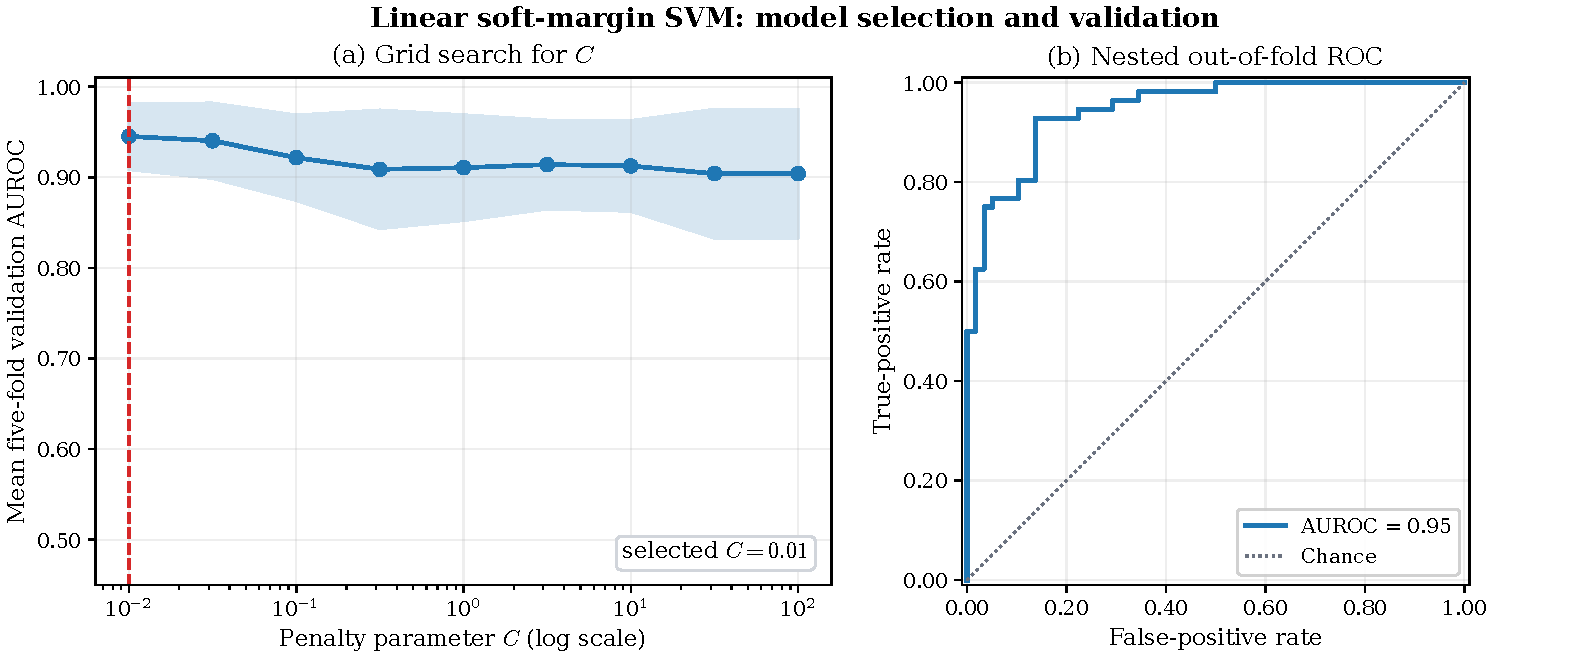
\includegraphics[width=\textwidth]{output/figures/linear_soft_margin_grid_roc.pdf}\\
      {\footnotesize (a) validation AUROC vs $C$; (b) nested out-of-fold ROC, \textbf{AUROC 0.95}.}
    \end{column}
  \end{columns}
\end{frame}

% ---------- 3a C grid search ----------
\begin{frame}{Step 3a --- choosing $C$ by grid search}
  \begin{columns}[T]
    \begin{column}{0.40\textwidth}
      Sweep $C$ over $10^{-2}\ldots10^{2}$ and score each by \textbf{inner-fold validation} AUROC (never the test fold --- leakage-safe).
      \vspace{0.5em}
      \begin{itemize}
        \item Training AUROC stays flat near $0.96$ at every $C$.
        \item Validation AUROC \emph{peaks at the smallest} $C=0.01$.
        \item Larger $C$ (harder penalty) $\Rightarrow$ worse generalization.
      \end{itemize}
      \vspace{0.4em}
      The gap between the two curves \emph{is} the overfitting.
    \end{column}
    \begin{column}{0.60\textwidth}
      \centering
      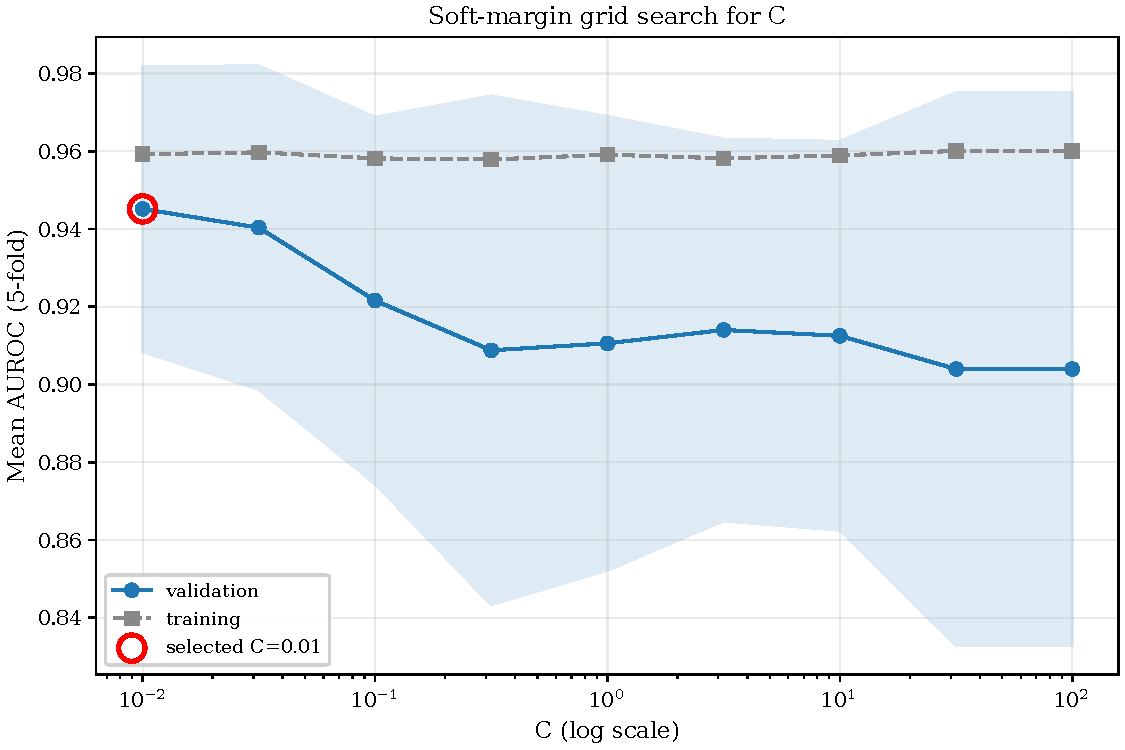
\includegraphics[width=\textwidth]{output/figures/fig_step3_c_grid.pdf}\\
      {\footnotesize Mean validation vs training AUROC across the $C$ grid; band is $\pm1$ SD over folds. The selected $C=0.01$ is circled.}
    \end{column}
  \end{columns}
  \take{Stronger regularization (small $C$) generalizes best on this overlapping data.}
\end{frame}

% ---------- 3b Pareto ----------
\begin{frame}{Step 3b --- the same grid as a Pareto trade-off}
  \begin{columns}[T]
    \begin{column}{0.40\textwidth}
      Plot each $C$ as (train--validation gap, validation AUROC). The best model is \textbf{top-left}: high AUROC \emph{and} little overfitting.
      \vspace{0.5em}
      \begin{itemize}
        \item $C=0.01$ is the \alert{single Pareto-optimal} point --- it wins on \emph{both} axes at once.
        \item Every larger $C$ gives away AUROC \emph{and} widens the gap.
        \item No trade-off to negotiate: the simplest penalty is strictly best here.
      \end{itemize}
    \end{column}
    \begin{column}{0.60\textwidth}
      \centering
      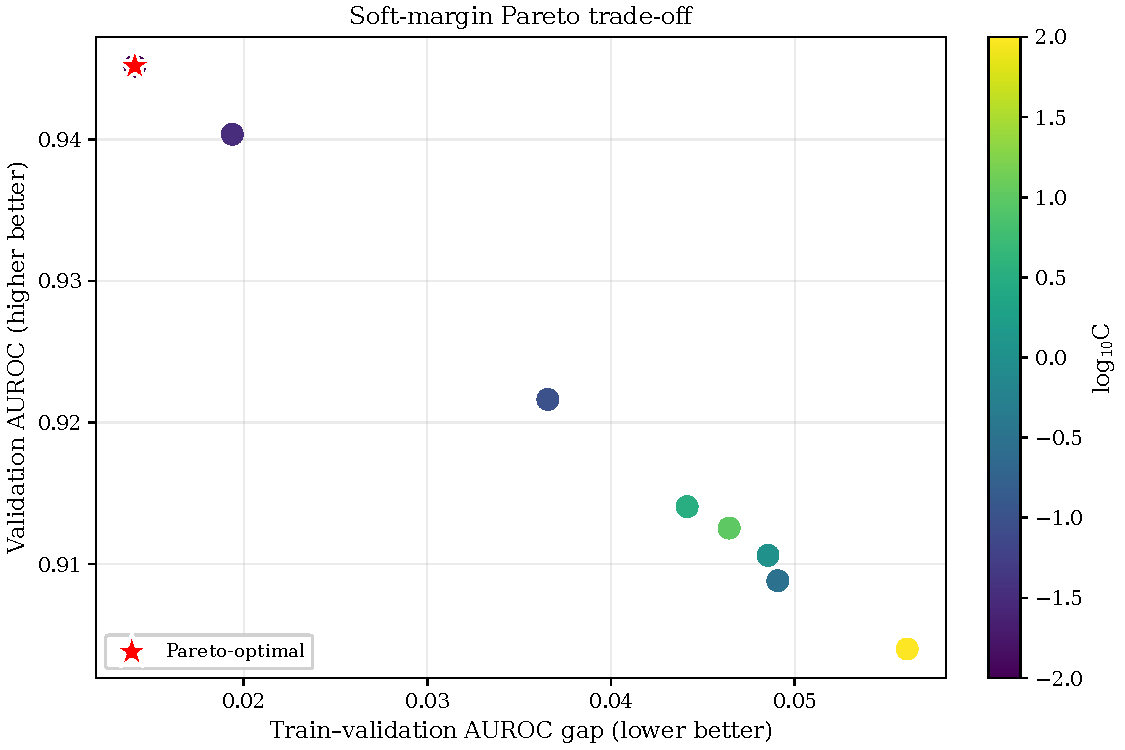
\includegraphics[width=\textwidth]{output/figures/fig_step3_pareto.pdf}\\
      {\footnotesize Color encodes $\log_{10}C$; the star is the selected, Pareto-optimal model.}
    \end{column}
  \end{columns}
  \take{$C=0.01$ dominates the grid on both axes at once.}
\end{frame}

% ---------- 3c PC-space decision boundary ----------
\begin{frame}{Step 3c --- what the soft-margin line looks like}
  \begin{columns}[T]
    \begin{column}{0.40\textwidth}
      Projecting the cohort onto its first two principal components makes the fitted \textbf{soft-margin boundary} visible.
      \vspace{0.5em}
      \begin{itemize}
        \item The line runs \emph{straight through the overlap} where the two hulls intersect.
        \item Circled points are \textbf{support vectors} --- almost all sit in the contested band.
        \item Points inside the margin or on the wrong side are exactly what the slack $\xi_i$ pays for.
      \end{itemize}
      \vspace{0.4em}
      {\footnotesize This 2-D fit is illustrative; the reported model uses all 10 features.}
    \end{column}
    \begin{column}{0.60\textwidth}
      \centering
      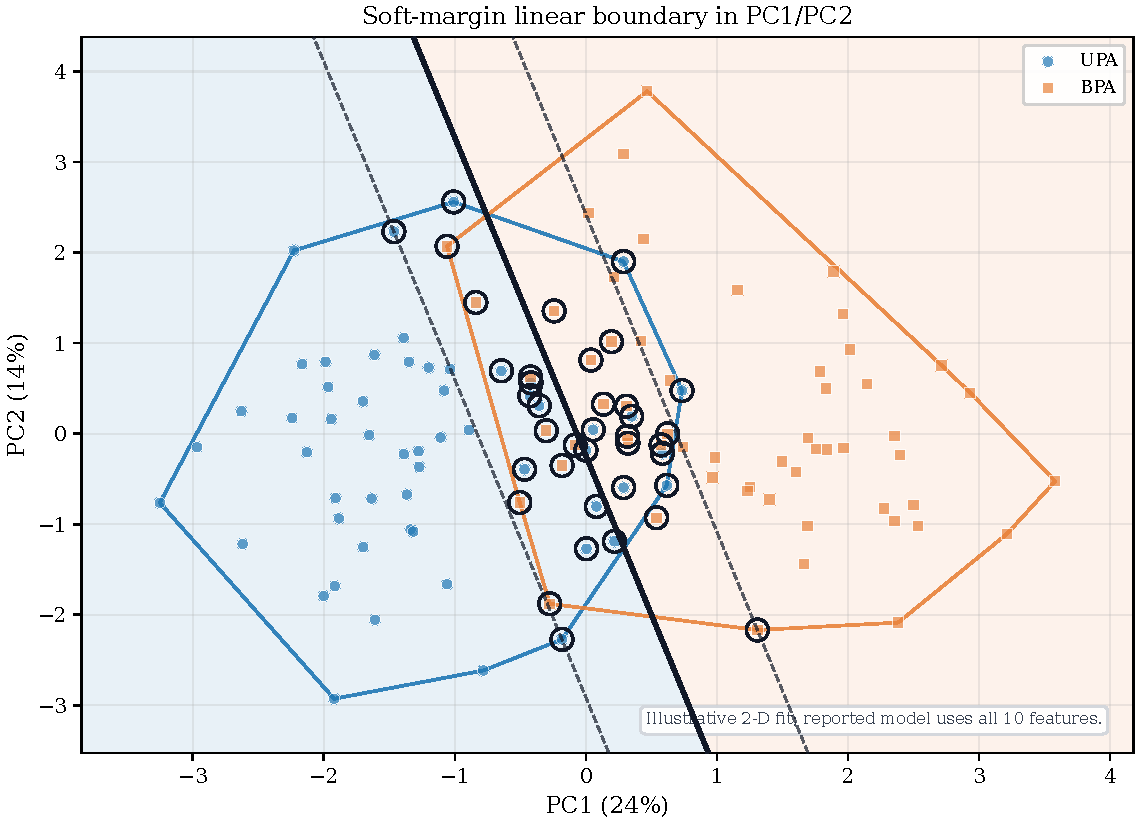
\includegraphics[width=\textwidth]{output/figures/fig_step3c_pc_boundary.pdf}\\
      {\footnotesize Solid: decision boundary; dashed: the $\pm1$ margins. Hulls overlap, so no line separates them cleanly.}
    \end{column}
  \end{columns}
  \take{A separating line cannot avoid the overlap --- the soft margin accepts it and charges for it.}
\end{frame}

% ---------- RBF derivation ----------
\begin{frame}{Step 4 --- from soft margin to a kernel}
  \textbf{1. The soft-margin primal} (what we solved in Step 3):
  \[
    \min_{w,b,\xi}\ \tfrac12\lVert w\rVert^2 + C\sum_i \xi_i
    \quad\text{s.t.}\quad t_i(w^\top x_i+b)\ge 1-\xi_i,\ \ \xi_i\ge 0.
  \]
  \textbf{2. Its Lagrangian dual} --- the data enters \alert{only through inner products} $x_i^\top x_j$:
  \[
    \max_{\alpha}\ \sum_i \alpha_i - \tfrac12\sum_{i,j}\alpha_i\alpha_j\, t_i t_j\,\underbrace{x_i^\top x_j}_{\text{inner product}}
    \quad\text{s.t.}\quad 0\le\alpha_i\le C,\ \ \sum_i\alpha_i t_i = 0.
  \]
  \begin{columns}[T]
    \begin{column}{0.5\textwidth}
      \textbf{3. The kernel trick.} Map $x\!\mapsto\!\varphi(x)$ into a higher space and replace every inner product by a \textbf{kernel}:
      \[
        x_i^\top x_j \;\longrightarrow\; K(x_i,x_j)=\varphi(x_i)^\top\varphi(x_j).
      \]
    \end{column}
    \begin{column}{0.5\textwidth}
      \textbf{4. Choose the RBF kernel:}
      \[
        K(x_i,x_j)=\exp\!\big(-\gamma\lVert x_i-x_j\rVert^2\big).
      \]
      \small A curved boundary in the original space, still a convex QP in $\alpha$.
    \end{column}
  \end{columns}
  \vspace{0.3em}
  \begin{center}
    Decision score becomes \;$f(x)=\displaystyle\sum_i \alpha_i t_i\,K(x_i,x)+b$.
  \end{center}
  \take{Only the inner product changes --- everything else in the soft-margin problem stays put.}
\end{frame}

% ---------- RBF compare ----------
\begin{frame}{Step 4 --- compare against a curved boundary (RBF kernel)}
  \begin{columns}[T]
    \begin{column}{0.44\textwidth}
      The RBF kernel $K(x_i,x_j)=e^{-\gamma\lVert x_i-x_j\rVert^2}$ can bend the boundary.
      \vspace{0.5em}
      \begin{itemize}
        \item Joint search over 81 $(C,\gamma)$ pairs, nested CV.
        \item Best: $C=0.01,\ \gamma=0.001$ --- the \emph{smoothest} setting.
        \item Large $\gamma$: perfect training, near-chance validation (overfit).
      \end{itemize}
      \vspace{0.4em}
      The data wanted a nearly-straight boundary.
    \end{column}
    \begin{column}{0.56\textwidth}
      \centering
      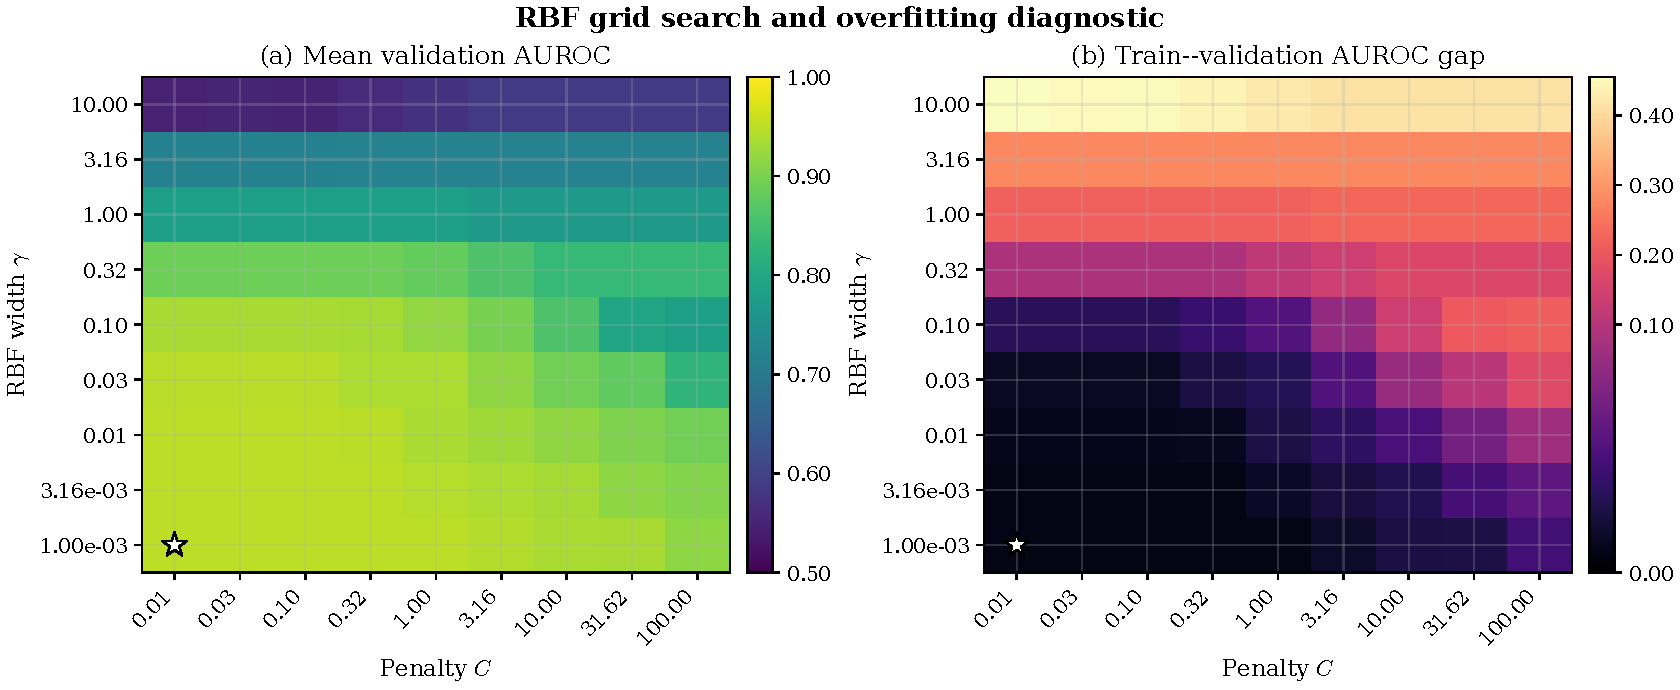
\includegraphics[width=\textwidth]{output/figures/rbf_kernel_grid_heatmaps.pdf}\\
      {\footnotesize Validation AUROC (left) vs train--validation gap (right). The star marks the selected smooth model; the top rows overfit.}
    \end{column}
  \end{columns}
\end{frame}

% ---------- Pareto frontier ----------
\begin{frame}{Step 4 --- performance versus overfitting: the Pareto view}
  \begin{columns}[T]
    \begin{column}{0.40\textwidth}
      Plot every candidate as (train--validation gap, validation AUROC). The \textbf{best models sit in the top-left}: high AUROC, small gap.
      \vspace{0.5em}
      \begin{itemize}
        \item \textcolor{UPAblue}{\textbf{Linear}}: the whole frontier is tightly clustered top-left --- little room to overfit.
        \item \textcolor{BPAorange}{\textbf{RBF}}: a long tail trades generalization for training fit as $\gamma$ grows.
        \item The Pareto-optimal RBF point coincides with the \emph{smoothest} setting --- essentially the linear model.
      \end{itemize}
    \end{column}
    \begin{column}{0.60\textwidth}
      \centering
      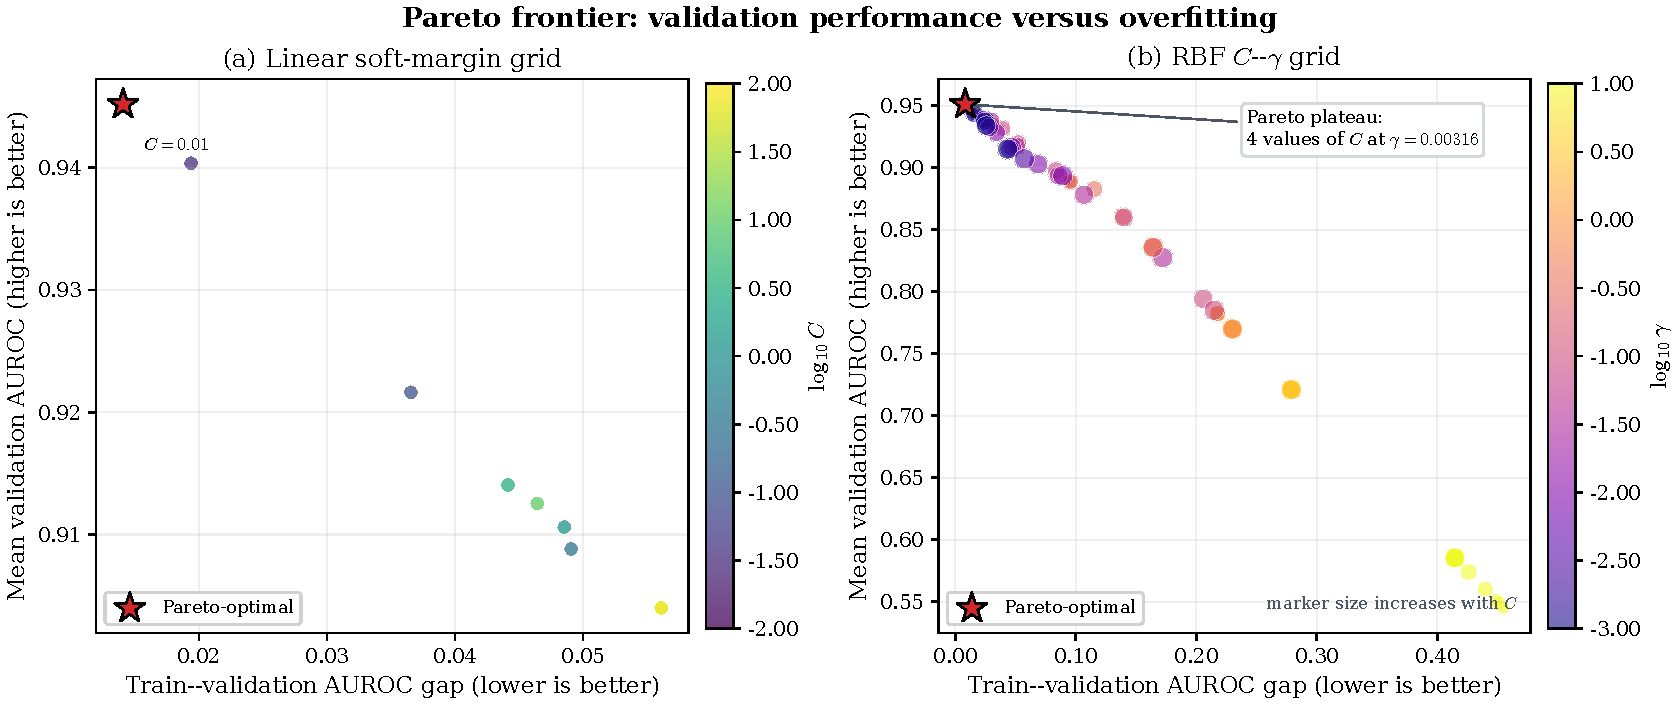
\includegraphics[width=\textwidth]{output/figures/svm_grid_pareto_frontier.pdf}\\
      {\footnotesize The star is the Pareto-optimal model in each grid. RBF's extra flexibility only buys a longer overfitting tail, not a better frontier.}
    \end{column}
  \end{columns}
  \take{More flexibility did not push the frontier outward --- it only added ways to overfit.}
\end{frame}

% ---------- Step 4 RBF PC-space boundary ----------
\begin{frame}{Step 4 --- the kernel boundary redrawn in PC1/PC2}
  \begin{columns}[T]
    \begin{column}{0.40\textwidth}
      The same projection as Step 3c, now with the \textbf{RBF-kernel} decision surface.
      \vspace{0.5em}
      \begin{itemize}
        \item The boundary is \alert{curved}, not straight --- the kernel's extra flexibility at work.
        \item It bends \emph{around} individual points, yet the two hulls still overlap.
        \item Curvature relabels a few borderline points but does not carve out a clean separation.
      \end{itemize}
      \vspace{0.4em}
      {\footnotesize Illustrative 2-D fit (moderate $\gamma$); the tuned model chose a much smoother $\gamma$.}
    \end{column}
    \begin{column}{0.60\textwidth}
      \centering
      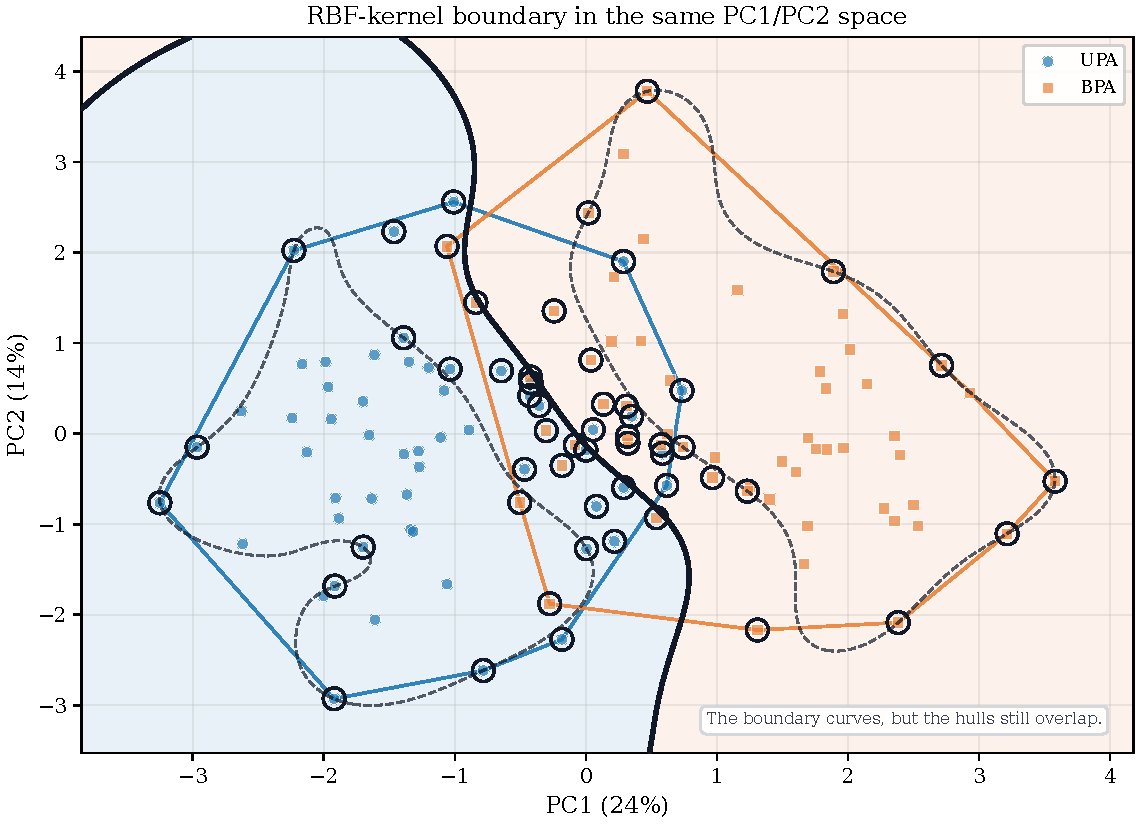
\includegraphics[width=\textwidth]{output/figures/fig_step4_rbf_pc_boundary.pdf}\\
      {\footnotesize Compare with the straight line of Step 3c: more shape, same overlap.}
    \end{column}
  \end{columns}
  \take{The kernel can bend the boundary --- but bending does not make overlapping classes separable.}
\end{frame}

% ---------- Statistical verdict ----------
\begin{frame}{Are linear and RBF actually different?}
  \begin{columns}[T]
    \begin{column}{0.55\textwidth}
      \centering
      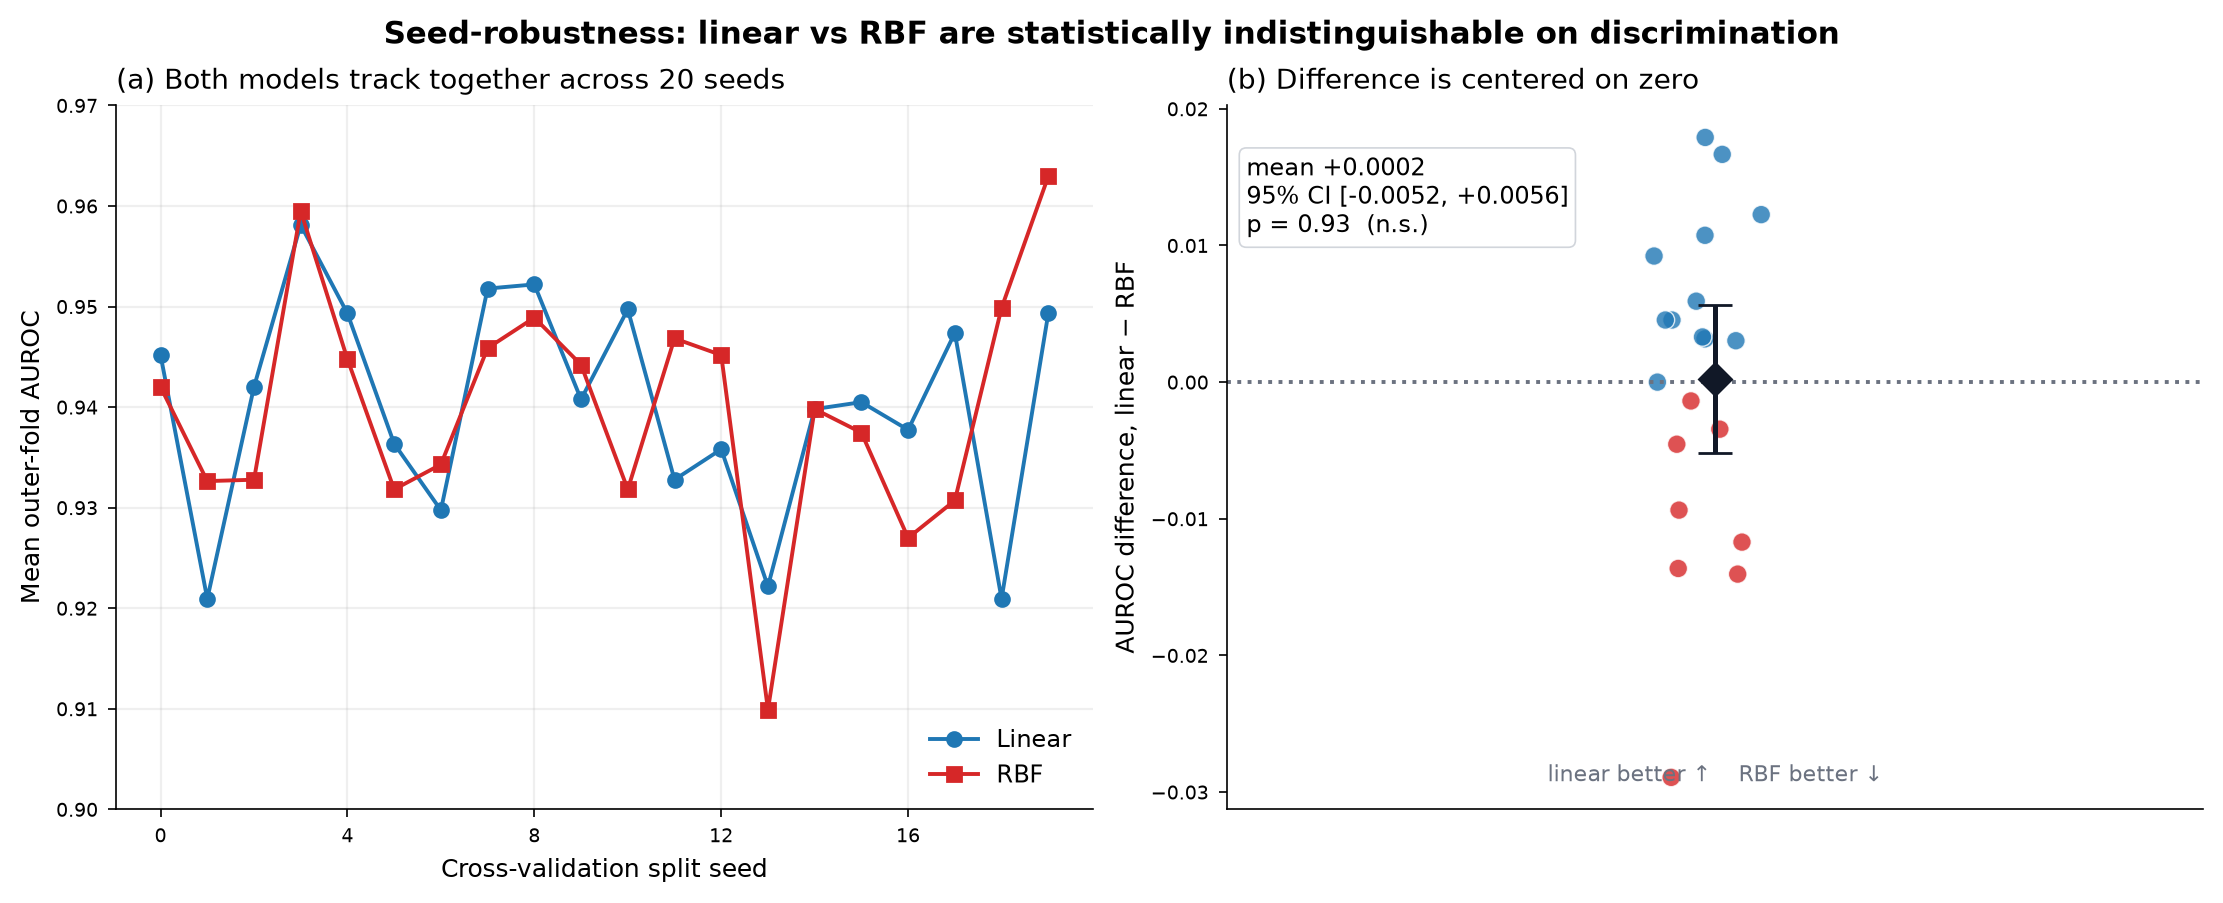
\includegraphics[width=\textwidth]{output/figures/fig_stat_seed_robustness.png}
    \end{column}
    \begin{column}{0.45\textwidth}
      \textbf{Fair metric} (mean outer-fold AUROC), 20 fold seeds:
      \begin{itemize}
        \item Difference $= +0.0002$
        \item 95\% CI $[-0.005,+0.006]$
        \item paired $t$: $p=0.93$ (n.s.)
        \item Linear $\ge$ RBF in 12/20 seeds.
      \end{itemize}
      \vspace{0.4em}
      \alert{Statistically indistinguishable} on discrimination.
    \end{column}
  \end{columns}
  \take{The kernel never improves on the line; the tiny gap is just the random split.}
\end{frame}

% ---------- Conclusion ----------
\begin{frame}{Step 5 --- conclude}
  \begin{columns}[T]
    \begin{column}{0.55\textwidth}
      \begin{block}{Verdict}
        \begin{itemize}
          \item Hard-margin $\to$ \textbf{impossible} (proven three ways).
          \item Linear soft-margin $\to$ \textbf{AUROC 0.95} \checkmark
          \item RBF kernel $\to$ AUROC 0.94 (no gain).
        \end{itemize}
        \vspace{0.3em}
        \textbf{The simpler model wins.}
      \end{block}
      Fewer tuning knobs, an interpretable score, equal discrimination --- parsimony decides.
    \end{column}
    \begin{column}{0.45\textwidth}
      \begin{block}{Why it matters}
        \small
        \begin{itemize}
          \item The negative feasibility result is \emph{informative}, not a bug: clinical measurements genuinely overlap.
          \item Complexity must be justified by \emph{validation}, never by training fit.
          \item Synthetic data $\Rightarrow$ methodological, not clinical, claim.
        \end{itemize}
      \end{block}
    \end{column}
  \end{columns}
\end{frame}

% ---------- Cheat-sheet backup ----------
\begin{frame}{One-page reference}
  \centering
  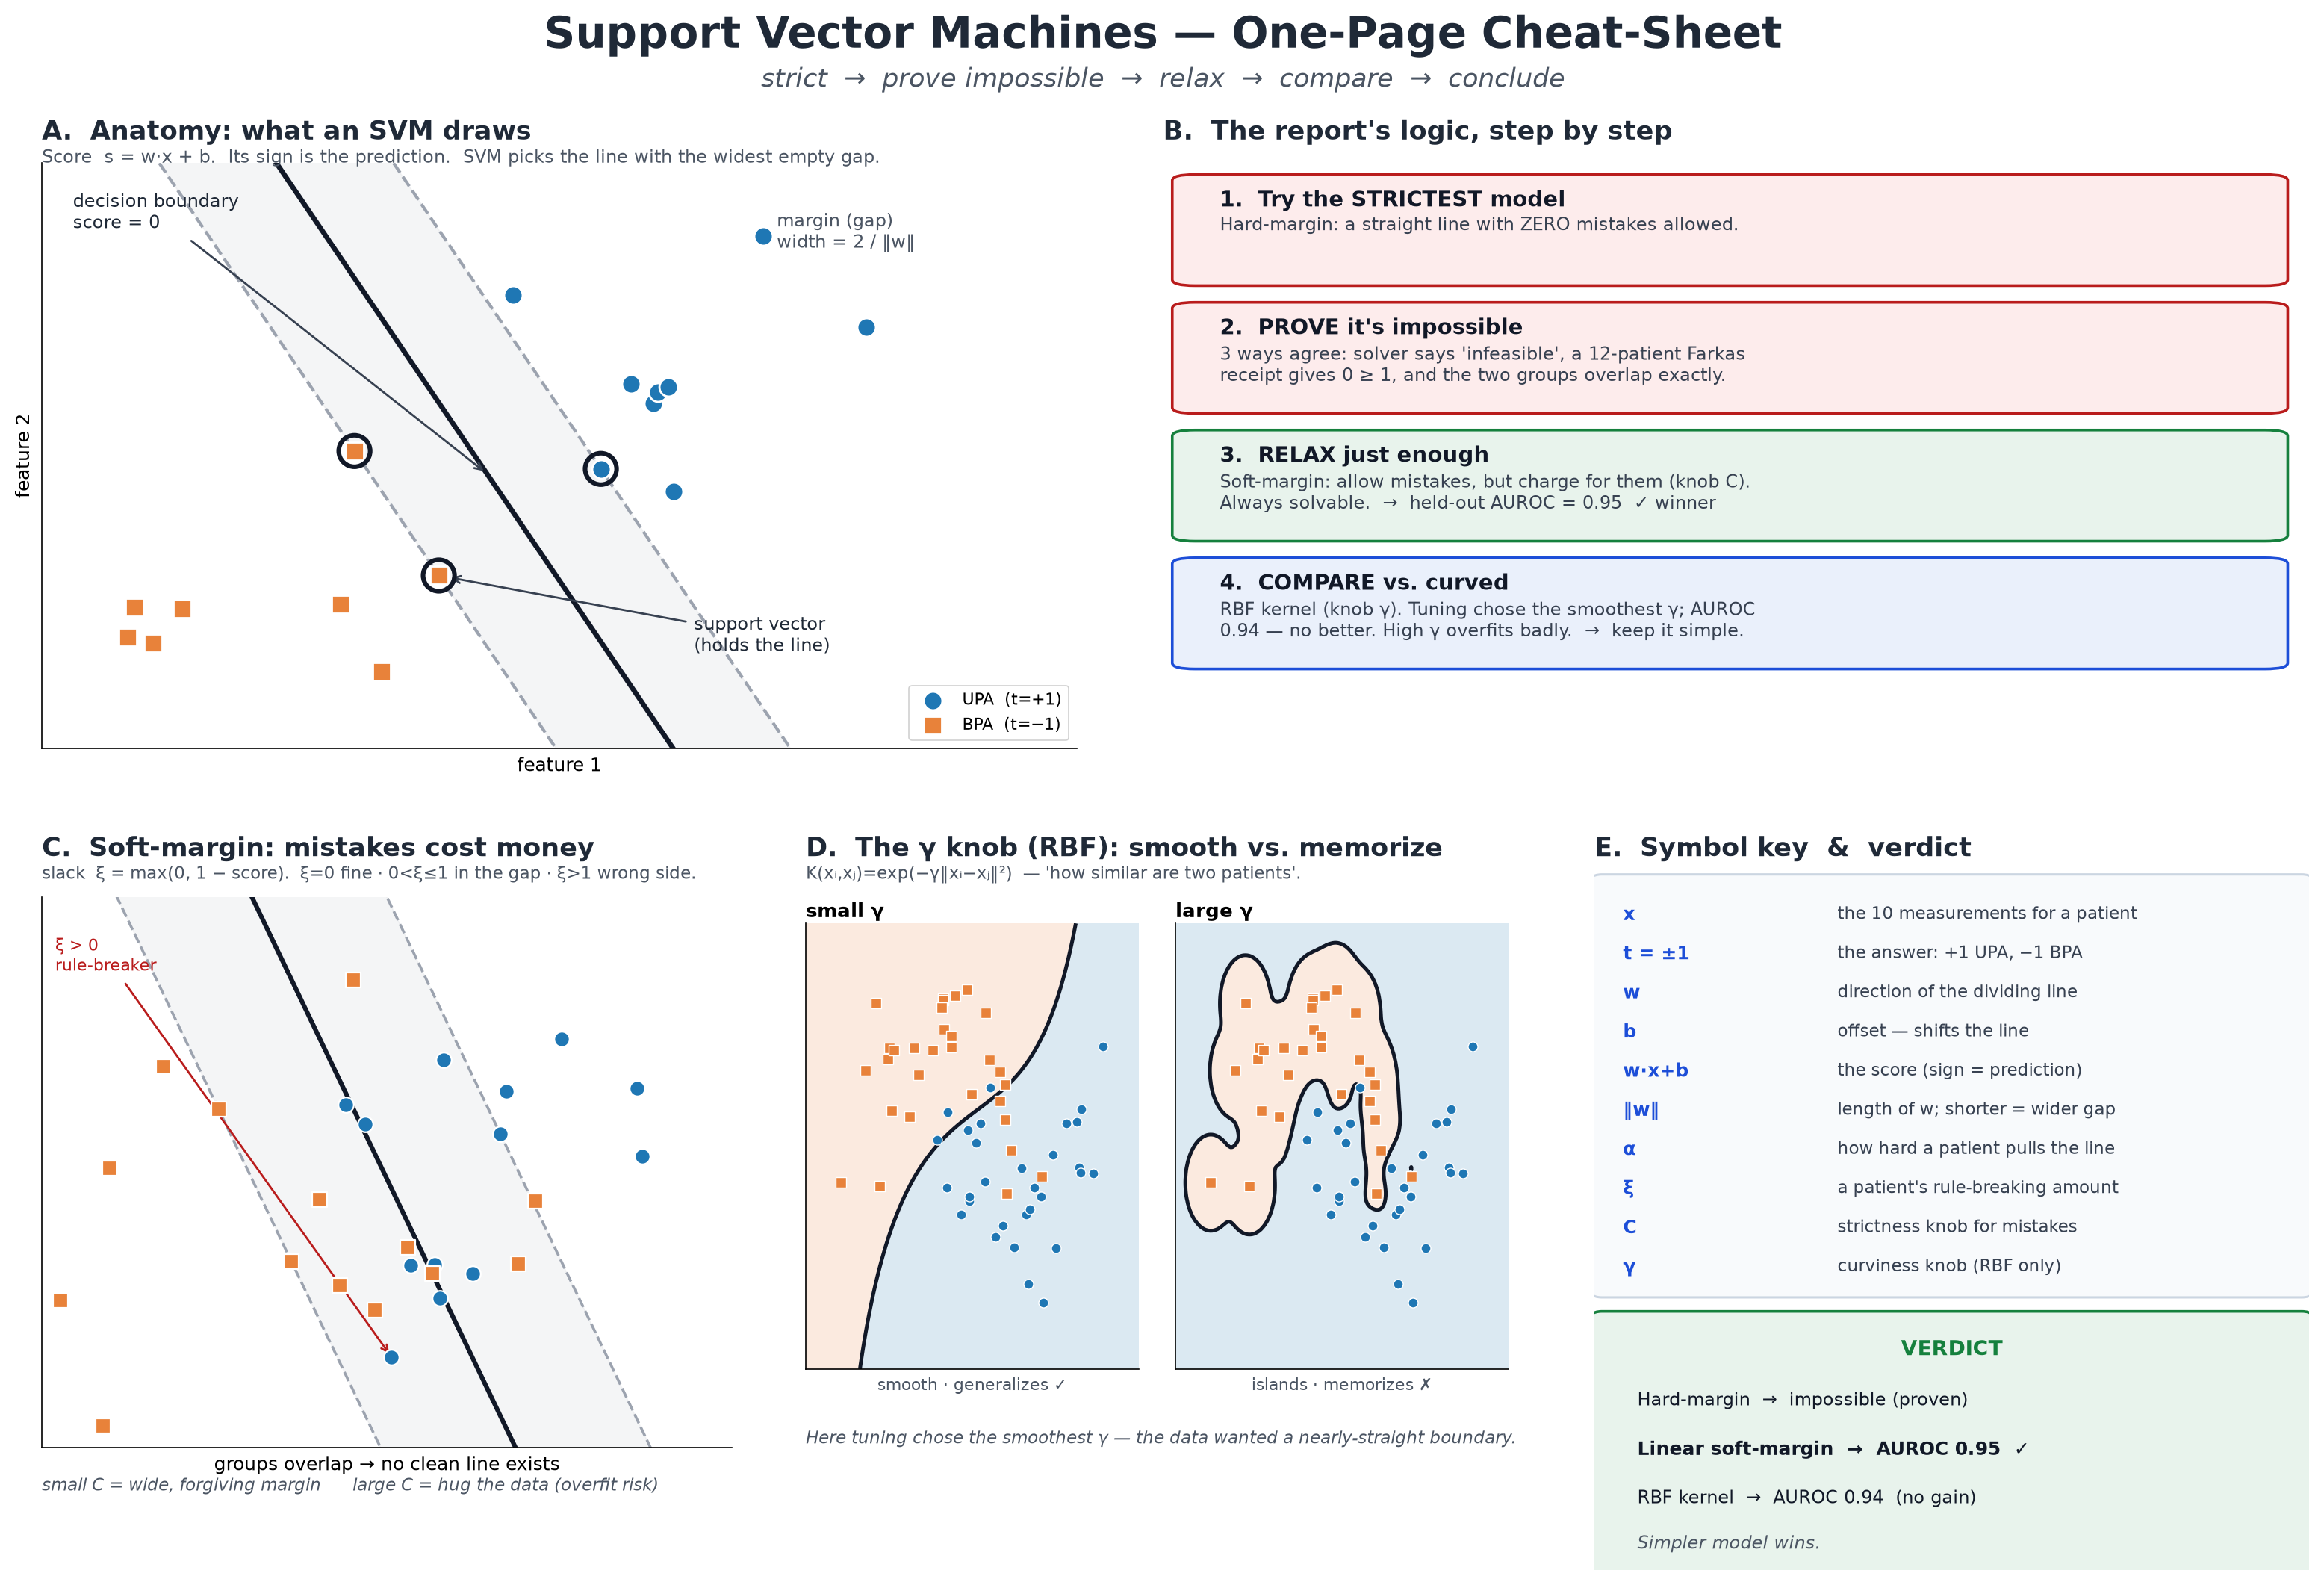
\includegraphics[height=0.86\textheight,keepaspectratio]{output/figures/fig_cheatsheet_ref.png}
\end{frame}

% ---------- Closing ----------
\begin{frame}[plain]
  \vfill
  \centering
  {\LARGE\bfseries\color{UPAblue} Thank you}\\[0.6em]
  {\large Questions?}\\[1.4em]
  {\footnotesize Reproduced end-to-end: 30/30 result files match; independent nested-CV and statistical tests confirm the verdict.}
  \vfill
\end{frame}

\end{document}